% ICCIT 2026 conference paper -- DysLex-Probe (8-page version)
% Build with XeLaTeX (Bangla glyphs need fontspec): xelatex conference.tex (run twice)
\documentclass[conference]{IEEEtran}

\usepackage{fontspec}
\setmainfont{TeX Gyre Termes}            % Times-compatible (IEEE look) under XeLaTeX
\newfontfamily\banglafont[Script=Bengali]{Noto Serif Bengali}
\newcommand{\bn}[1]{{\banglafont #1}}

\usepackage{amsmath,amssymb}
\usepackage{booktabs}
\usepackage{array}
\usepackage{graphicx}
\graphicspath{{figs/}}
\usepackage{url}
\usepackage[hidelinks]{hyperref}

\begin{document}

\title{Surface-Controlled Cross-Lingual Lexical Probing of Multilingual LLMs for Low-Resource Bangla Dyslexia Screening}

\author{
\IEEEauthorblockN{Ayesha Siddika, Nazmoon Nahar Aka, Mashrafi Rahman, Hasan Mohammad Sayem}
\IEEEauthorblockA{\textit{Department of Computer Science and Engineering} \\
\textit{BRAC University}\\
Dhaka, Bangladesh}
\and
\IEEEauthorblockN{Dr.\ Farig Yousuf Sadeque, Md.\ Tanzim Reza}
\IEEEauthorblockA{\textit{Department of Computer Science and Engineering} \\
\textit{BRAC University}\\
Dhaka, Bangladesh}
}

\maketitle

\begin{abstract}
Dyslexia screening in low-resource languages is constrained by the scarcity of expert clinicians, validated test batteries and labelled corpora. Multilingual large language models (LLMs) are an attractive substrate because their pretraining already encodes cross-lingual structure, but it is not known which architectures actually carry lexical and phonological information that transfers from a high-resource source (English) to a low-resource target (Bangla), nor where in the network that information resides. We probe four publicly released multilingual LLMs spanning the four dominant pretraining recipes -- XLM-RoBERTa large (multilingual masked encoder), Llama~3.1 8B (English-heavy causal decoder), BLOOM 7B1 (multilingual causal decoder) and mT5 XL (multilingual span-corruption encoder-decoder) -- with frozen per-layer linear probes on a curated 440-item English/Bangla stimulus set. A central methodological finding is that three of four standard phonological probing tasks fail surface-feature sanity checks: Bangla voicing labels are recoverable from the first character alone (F1 0.78--0.94), and orthographic and syllable probes do not exceed a five-feature character-statistic baseline. After 1:1 character-length matching, only real-versus-pseudo word discrimination survives; on it, BLOOM reaches 0.92 F1 and XLM-R 0.86 F1 on zero-shot Bangla transfer, while Llama (0.63) and mT5 (0.60) collapse to surface level. A 0.56B multilingual encoder thus outperforms an 8B English-heavy decoder. Causal forward-hook ablation shows that mT5 alone localises the cross-lingual signal to a small set of encoder units (specificity $+0.11$), with two backbone units persisting across encoder depth. Pretraining objective and language coverage, not parameter scale, determine cross-lingual lexical transfer.
\end{abstract}

\begin{IEEEkeywords}
multilingual language models, cross-lingual transfer, probing classifiers, dyslexia screening, low-resource Bangla NLP, representational similarity analysis, causal ablation, mechanistic interpretability
\end{IEEEkeywords}

\section{Introduction}
Developmental dyslexia is a specific learning difficulty that impairs accurate and fluent word reading, decoding and spelling despite adequate intelligence, schooling and sensory function \cite{snowling2020dyslexia,peterson2012developmental}. Estimated prevalence ranges from five to twelve percent of school-age children depending on language and writing system \cite{ziegler2005reading,wagner2020prevalence}, and the dominant cognitive account is the \emph{phonological deficit hypothesis}: dyslexic readers are weaker at representing, retrieving and manipulating speech sounds, which slows grapheme-to-phoneme mapping during reading acquisition \cite{snowling2020dyslexia,goswami2011temporal}.

Clinical identification depends on standardised, language-specific test batteries such as CTOPP-2 \cite{wagner2013ctopp}, which require trained psychometricians and do not exist for most of the world's languages. Bangla, with more than 270 million speakers, has no widely deployed normative dyslexia screener and no consensus diagnostic battery \cite{nag2014dyslexia,nag2017indian,badsha2024mall}; suspected cases are identified late or not at all. The absence of such norms is itself a barrier to identification and is a primary motivation for this work.

In parallel, multilingual LLMs have crossed a capability threshold at which their hidden representations encode rich, transferable linguistic structure across the languages in their pretraining mix \cite{conneau2020xlmr,scao2022bloom,xue2021mt5}. The same models that drive translation and dialogue are accumulating, as a by-product, the lexical and sub-lexical structure that clinical screening tools probe explicitly. If that structure transfers from a resource-rich language (English, where validated probes and labels exist) to a low-resource language (Bangla, where they do not), a single multilingual model could anchor a family of screening prototypes across many languages at once. A genuine phonological representation should generalise across orthographic depth; surface statistics should not.

However, much prior probing work uses \emph{unmatched} stimuli, leaving surface confounds such as character length, byte length and first-character identity uncontrolled. A probe that appears to ``recover voicing'' may simply be reading the first character of the word. Whether the reported cross-lingual phonological effects survive tight surface controls is, to our knowledge, untested across architectures.

This paper makes three contributions.
\begin{enumerate}
\item \textbf{Methodological.} Under first-character, character-statistic and length-matching controls, three of four standard phonological probing tasks are shown to measure surface artefacts rather than phonology. Surface-matched stimuli and native-verified labels are the minimum standard for cross-lingual clinical probing.
\item \textbf{Comparative.} Across the four canonical pretraining recipes, only multilingual models with explicit Bangla coverage achieve genuine cross-lingual lexical transfer; a 0.56B multilingual encoder beats an 8B English-heavy decoder, so coverage and objective dominate scale.
\item \textbf{Interpretability.} Only the encoder-decoder model (mT5) localises the cross-lingual lexical signal to a small set of encoder units, with a persistent backbone across depth, whereas the other models distribute it.
\end{enumerate}

\section{Background and Related Work}
\subsection{Dyslexia and the phonological deficit}
The phonological deficit hypothesis holds that the core impairment in dyslexia is in the phonological component of language \cite{snowling2020dyslexia,goswami2011temporal}. Behaviourally, the strongest single marker is impaired \emph{pseudoword reading}: because a pseudoword has no lexical entry, it can only be read by phonological decoding, isolating exactly the skill that breaks down in dyslexia. This motivates a probing design centred on real-versus-pseudoword discrimination and on sound-contrast (minimal-pair) items.

\subsection{Orthographic depth and Bangla}
Orthographic depth -- how directly spelling maps to sound -- predicts cross-language differences in reading acquisition and dyslexia manifestation \cite{ziegler2005reading}. English is orthographically opaque; Bangla is intermediate, with a largely regular consonant inventory but heavy use of conjunct characters (\textit{yuktoborno}) and vowel diacritics (\textit{matra}) that do not transparently decompose. This makes the English-to-Bangla direction a natural cross-lingual testbed: a representation that survives the change of script and depth is encoding structure rather than surface form. The Bangla difficulty patterns documented by Badsha \cite{badsha2024mall} for dyslexic Bangla-speaking children -- voiced/unvoiced confusions, aspiration, conjuncts and multisyllabic load -- ground our Bangla stimulus design.

\subsection{Multilingual LLMs and pretraining recipes}
Modern multilingual LLMs differ along two axes that this study isolates: pretraining objective and language coverage. XLM-RoBERTa \cite{conneau2020xlmr} is a multilingual masked encoder; BLOOM \cite{scao2022bloom} and Llama~3.1 \cite{dubey2024llama3} are causal decoders differing chiefly in coverage (BLOOM is explicitly multilingual, Llama is English-heavy); mT5 \cite{xue2021mt5} is a multilingual span-corruption encoder-decoder. Multilingual encoders are known to exhibit emergent cross-lingual structure \cite{pires2019mbert,wu2020emerging}, but coverage across languages is uneven, and it is unclear how much of the apparent transfer is surface-driven.

\subsection{Probing and interpretability}
Linear probing reads target properties from frozen representations with low-capacity classifiers, so success implies the property is linearly available rather than learned by the probe \cite{conneau2018probing,hewitt2019structural,belinkov2022probing}. The central methodological risk is that probes succeed on confounds rather than the intended property \cite{belinkov2022probing,pimentel2020information}; control baselines are therefore essential. Beyond probing, causal interventions (ablating units and measuring the effect) test whether information is merely decodable or causally used, and Representational Similarity Analysis (RSA) compares representational geometry without training any probe.

\subsection{Automated dyslexia screening}
Prior computational approaches to dyslexia screening have largely relied on task-specific behavioural signals: supervised models over handwriting samples, eye-tracking during reading, gameplay telemetry, or audio of oral reading, typically trained per language on labelled child data. Such pipelines are accurate where data exist but do not transfer to languages without labelled corpora, which is the situation for Bangla. Our approach is complementary and upstream: rather than training a screener, we ask whether the representations of an already-pretrained multilingual model contain the phonological and lexical structure that such a screener would need, and whether that structure transfers across languages. A positive answer identifies a substrate on which a downstream, clinician-supervised screener can later be built without per-language pretraining.

\subsection{Research gap}
We are not aware of prior work that compares the four dominant multilingual pretraining recipes on the same surface-controlled cross-lingual lexical task, with the same stimuli and metrics, and then localises the signal causally. This study closes that gap and frames it around a concrete low-resource application.

\section{Stimulus Dataset}
\subsection{Design principles}
The dataset is a single 440-item CSV (220 English + 220 Bangla, 18 metadata columns), identical across all four model runs so that any difference is attributable to the models. It is perfectly balanced by language and balanced by category within language, the categories map onto documented dyslexia error types, and the rich metadata exists specifically to support confound control.

\subsection{Categories and counts}
The dataset contains seven phonological task categories (200 items per language) plus a 40-item cross-lingual concept-matching set used for RSA (Table~\ref{tab:data}). Minimal pairs probe one-sound contrasts; pseudowords isolate decoding; real words are length-matched to pseudowords; phoneme-grapheme, rhyme, multisyllabic and sentence items probe further phonological skills. Bangla items are stored in Unicode Bengali script, e.g.\ real word \bn{পানি} (``water''), minimal pair \bn{কাল}/\bn{গাল}, pseudoword \bn{নিদা}, conjunct-bearing sentence \bn{সে স্কুলে যায়।}

\begin{table}[t]
\caption{Per-category stimulus counts (English / Bangla).}
\label{tab:data}
\centering
\small
\setlength{\tabcolsep}{3.5pt}
\begin{tabular}{lccc}
\toprule
\textbf{Category} & \textbf{EN} & \textbf{BN} & \textbf{Total} \\
\midrule
Minimal pair        & 60 & 60 & 120 \\
Multisyllabic       & 30 & 30 & 60 \\
Pseudoword          & 25 & 25 & 50 \\
Real word           & 25 & 25 & 50 \\
Phoneme-grapheme    & 25 & 25 & 50 \\
Rhyme               & 20 & 20 & 40 \\
Sentence            & 15 & 15 & 30 \\
\textit{Phonological subtotal} & \textit{200} & \textit{200} & \textit{400} \\
Concept match (RSA) & 20 & 20 & 40 \\
\midrule
\textbf{Total}      & \textbf{220} & \textbf{220} & \textbf{440} \\
\bottomrule
\end{tabular}
\end{table}

\subsection{Bangla grounding and verification}
Three elements of the Bangla design are taken directly from Badsha \cite{badsha2024mall}: the five voiced/unvoiced stop pairs (\bn{ক/গ}, \bn{প/ব}, \bn{ত/দ}, \bn{ট/ড}, \bn{চ/জ}) used as Bangla minimal pairs, the multisyllabic and \textit{matra} error patterns, and the human difficulty ranking (voicing hardest, syllable count easiest). All Bangla items were inspected by a native speaker for orthographic validity; Bangla pseudowords follow Bangla phonotactics and were re-checked to remove accidental real words.

\subsection{Metadata and length matching}
Each item carries 18 columns including IPA, syllable count, phonological complexity, orthographic transparency, consonant-cluster and irregular-mapping flags, and the targeted dyslexia error type. All length-based controls are computed on the original Unicode string, not the tokeniser output, to avoid tokeniser bias from conjunct decomposition. For surface-controlled reporting we use a real-versus-pseudoword subset matched 1:1 on character length, $n=50$ per language (mean characters EN 6.88, BN 5.20), selected deterministically (\texttt{random\_state=42}).

\section{Methodology}
\subsection{Models}
We probe four publicly released multilingual LLMs (Table~\ref{tab:models}) chosen to exhaust the design grid \{encoder-only, decoder-only, encoder-decoder\} $\times$ \{multilingual, English-heavy\} at consumer-GPU scale. The two 7--8B decoders use 4-bit quantised inference \cite{dettmers2022bnb}; XLM-R and the mT5 encoder run in 16-bit. For mT5 only the encoder is probed. All models are frozen, with no parameter update.

\begin{table}[t]
\caption{Probed multilingual LLMs. For mT5 only the 1.67B encoder is used.}
\label{tab:models}
\centering
\small
\setlength{\tabcolsep}{4pt}
\begin{tabular}{lccccc}
\toprule
\textbf{Model} & \textbf{Architecture} & \textbf{Tok.} & \textbf{Params} & \textbf{Layers} & \textbf{Bangla} \\
\midrule
XLM-R large  & encoder-only    & SP   & 0.56B & 24 & explicit \\
Llama 3.1 8B & decoder-only    & BPE  & 8B    & 32 & minimal \\
BLOOM 7B1    & decoder-only    & BPE  & 7.1B  & 30 & explicit \\
mT5 XL       & enc-decoder     & SP   & 3.7B  & 24 & explicit \\
\bottomrule
\end{tabular}
\end{table}

\subsection{Model details}
Figure~\ref{fig:models} compares the four architectures side by side. \textbf{XLM-R large} is a 24-layer bidirectional masked encoder with a 250k-token SentencePiece vocabulary built jointly over 100 languages, so Bangla conjuncts are tokenised into subwords rather than discarded; we mean-pool the non-special tokens to a 1024-d vector per layer and run it in 16-bit without quantisation. \textbf{Llama 3.1 8B} is a 32-layer causal decoder with an English-tuned tiktoken BPE that handles Bangla at the byte level; it is run in 4-bit and pooled to 4096-d. \textbf{BLOOM 7B1} is a 30-layer causal decoder whose BPE was trained jointly on the 46-language ROOTS corpus, so Bangla subwords are first-class; its pipeline mirrors Llama exactly so that any difference is attributable to coverage, not instrumentation. \textbf{mT5 XL} contributes only its 24-layer span-corruption encoder (the decoder is loaded but never invoked); it is bidirectional, runs in 16-bit, and at 1.67B encoder parameters is the highest-fidelity model, which is why the compute-intensive depth-scan ablation is run on it specifically.

\begin{figure*}[t]
\centering
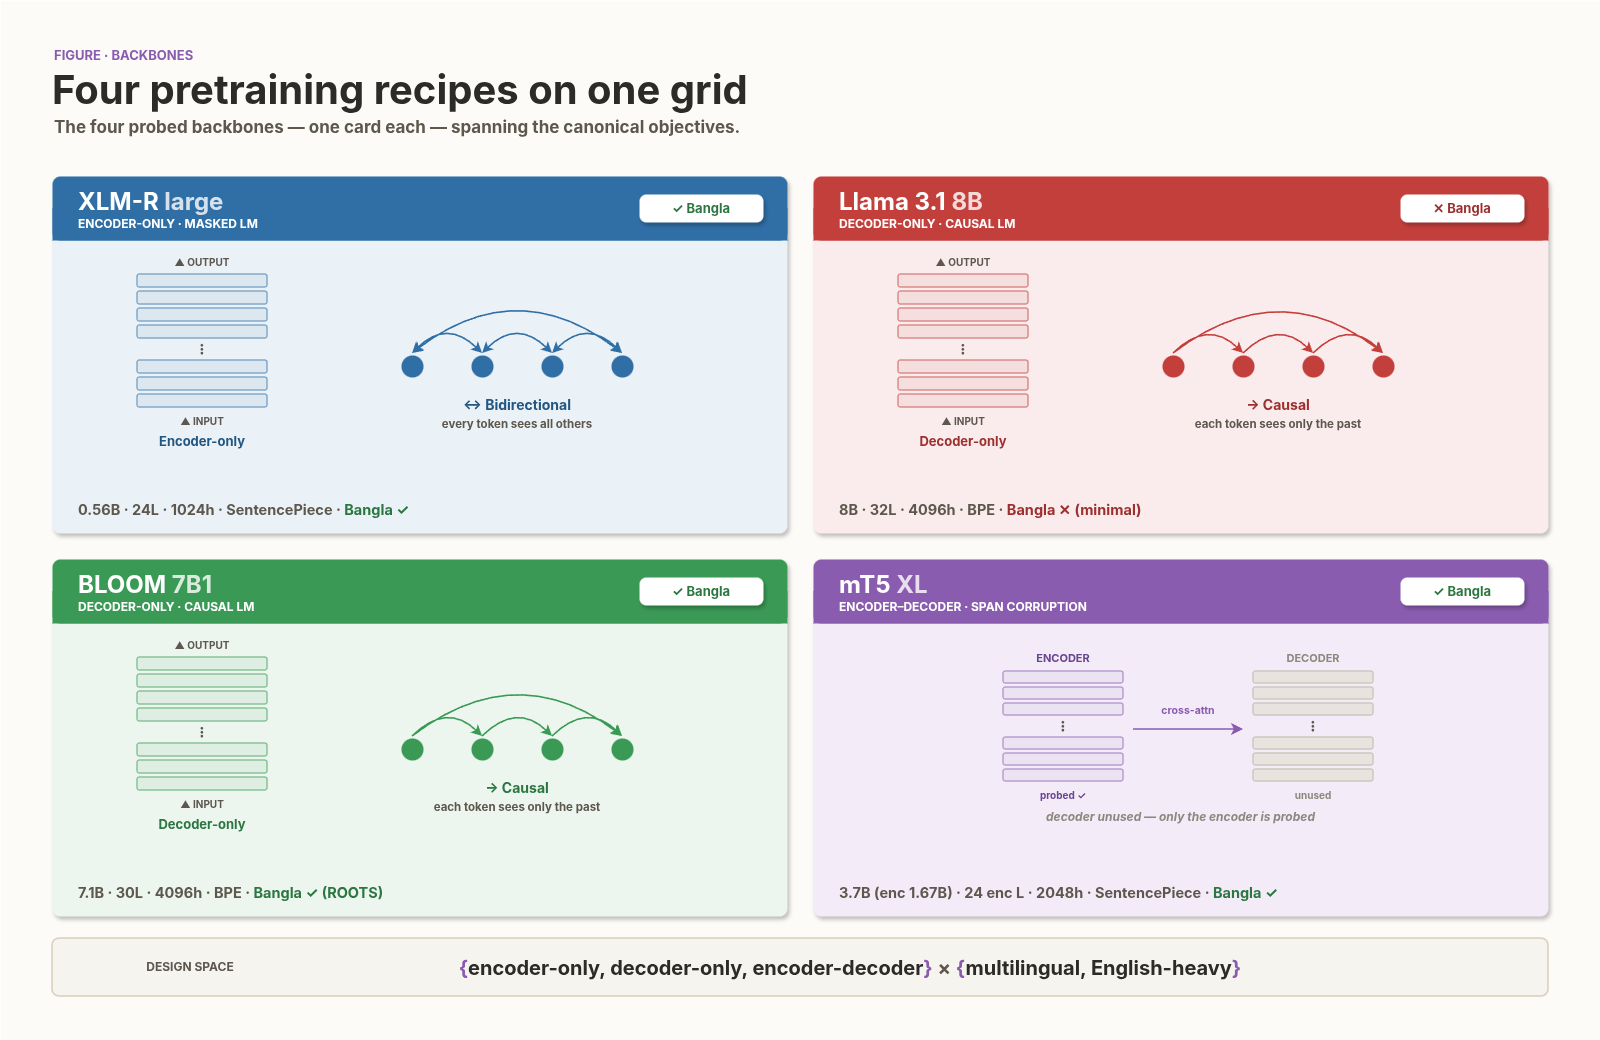
\includegraphics[width=0.95\textwidth]{fig_models.png}
\caption{Architectural comparison of the four probed multilingual LLMs. XLM-R is a multilingual masked encoder (bidirectional); Llama and BLOOM are causal decoders differing chiefly in language coverage; mT5 is a span-corruption encoder-decoder whose decoder is unused (only the encoder is probed). Parameter count, layer count, hidden size, tokeniser and Bangla coverage are annotated per model.}
\label{fig:models}
\end{figure*}

\subsection{Frozen per-layer linear probing}
Each stimulus is passed through the frozen model in a single forward pass; per-layer hidden states are mean-pooled across input tokens to one vector per layer. A per-layer linear probe (logistic regression for classification, ridge regression for syllable count) is trained on English representations and evaluated on held-out English (in-language) and on Bangla (zero-shot cross-lingual). We report macro-F1 for classification and $R^2$ for regression, averaged over five-fold cross-validation within the English split for layer-selection robustness. Figure~\ref{fig:pipeline} summarises the end-to-end pipeline.

\begin{figure}[t]
\centering
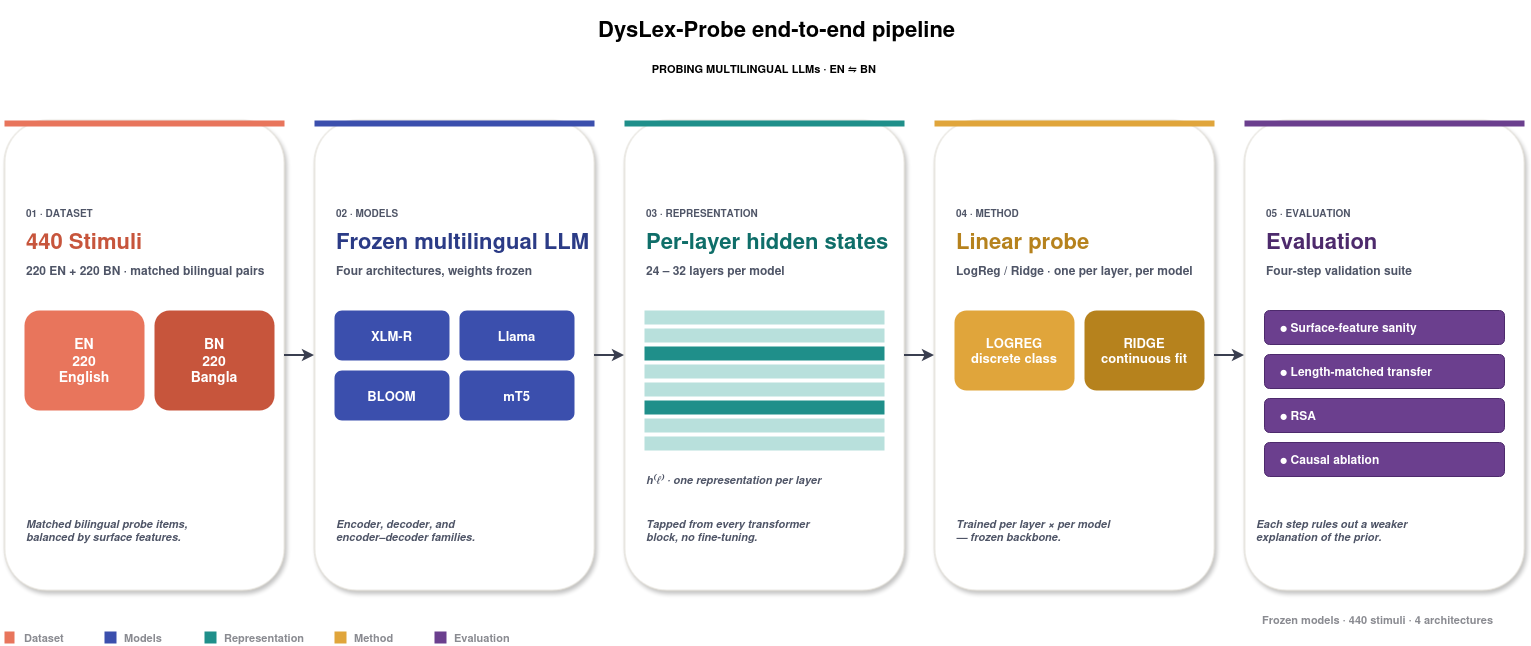
\includegraphics[width=0.96\columnwidth]{fig_pipeline.png}
\caption{End-to-end probing pipeline. The 440-item English/Bangla dataset is fed through each frozen multilingual LLM; per-layer hidden states are extracted, a linear probe is trained on English, and representations are evaluated under surface-feature sanity checks, length-matched cross-lingual transfer, RSA and causal forward-hook ablation.}
\label{fig:pipeline}
\end{figure}

\subsection{Probing tasks and labels}
Four label sets are probed. \emph{Voicing} is binary \{voiced, unvoiced\}, applied to minimal-pair and real-word items whose leading stop consonant has a clear voicing class. \emph{Real-versus-pseudo word} is binary \{real, pseudo\}, applied to the union of the real-word and pseudoword categories and, for surface-controlled reporting, to their length-matched subset. \emph{Orthographic transparency} is binary \{transparent, opaque\}, assigned per item from orthographic-mapping rules. \emph{Syllable count} is an integer regression target (word count for sentences). Each task is probed at every layer of every model, and the per-layer peak is selected by cross-validation within the English training split to avoid peeking at the Bangla test side.

\subsection{Surface-feature sanity controls}
Three controls gate every claim. (i) A \emph{first-character lookup} baseline: a leave-one-out probe trained on the layer-0 token embedding with a one-hot encoding of the first character, quantifying how much of a label is recoverable from the first character alone. (ii) A \emph{five-feature character-statistic} baseline (character length, byte length, unique-character count, vowel ratio, longest consonant run); any LLM probe that does not exceed this by more than 0.03 is treated as contributing no information above surface statistics. (iii) \emph{1:1 character-length matching} of real and pseudo words. The unit of evidence throughout is gain-over-surface, not gain-over-chance.

\subsection{Representational Similarity Analysis}
On the cross-lingual concept-match pairs we compute, per layer, the cosine Representational Dissimilarity Matrix (RDM) within each language and correlate the English and Bangla RDMs by Spearman $\rho$; we also report English$\to$Bangla mate-retrieval Top-1 accuracy. RSA requires no probe training and so corroborates the probing result with an independent, geometry-only measure.

\subsection{Causal forward-hook ablation}
On the surviving task we zero the top-$K$ probe-ranked hidden units via forward hooks and remeasure Bangla transfer, against a random-unit control with multiple seeds. \emph{Specificity} is the ranked-unit drop minus the random-unit drop; a positive value indicates the information is concentrated in those units. The mT5 encoder is re-ablated at five depths (\texttt{measure\_L} $\in\{4,8,12,16,20\}$) with three seeds each, and we measure the Jaccard overlap of the top-ranked units across depths to test for persistent ``backbone'' units.

\subsection{Reproducibility}
Every reported number corresponds to a deterministic CSV in a per-model results directory, with fixed seeds for probe training (\texttt{random\_state=42}) and three seeds for ablation random-unit controls. Probes use L2-regularised logistic/ridge regression with fixed train/test splits and majority-class (classification) and mean-predictor (regression) chance baselines. The four-model integration is emitted to a single comparison artefact, and pinned library and CUDA versions are recorded so the study is regenerable end to end on a single consumer GPU.

\section{Results}
\subsection{RQ1: most standard tasks fail sanity checks}
In-language English probing recovers all four tasks at first sight (Table~\ref{tab:rq1}), but the sanity checks reframe three of them. Bangla voicing labels are 100\% recoverable from the first character: a layer-0 leave-one-out probe scores F1 0.78--0.94 across the four models (Table~\ref{tab:sanity}), so the probe reads letter identity, not phonological voicing. Orthographic transparency is solved by the five-feature surface baseline (EN F1 0.66, BN 0.82), with the LLMs adding at most $+0.03$. Syllable count is surface-confounded (EN surface $R^2$ 0.81), and three of four models fall below the surface baseline. Only real-versus-pseudo word survives.

\begin{table}[t]
\caption{RQ1 in-language English probing: peak layer / peak score per model per task (F1; $R^2$ for syllable). Daggered tasks fail surface-feature sanity checks.}
\label{tab:rq1}
\centering
\small
\setlength{\tabcolsep}{4pt}
\begin{tabular}{lcccc}
\toprule
\textbf{Task} & \textbf{XLM-R} & \textbf{Llama} & \textbf{BLOOM} & \textbf{mT5} \\
\midrule
Voicing$^\dagger$    & L11/0.62 & L2/0.73  & L6/0.55  & L9/0.58  \\
Realword             & L11/0.84 & L12/0.91 & L22/0.79 & L24/0.81 \\
Ortho$^\dagger$      & L0/0.92  & L32/0.71 & L12/0.68 & L21/0.69 \\
Syllable$^\dagger$   & L8/0.67  & L16/0.70 & L29/0.68 & L20/0.76 \\
\bottomrule
\end{tabular}
\end{table}

\begin{table}[t]
\caption{First-character sanity check (Bangla voicing): leave-one-out F1 at layer~0 versus peak, with the deterministic upper bound. The label is recoverable from the first character alone.}
\label{tab:sanity}
\centering
\small
\setlength{\tabcolsep}{5pt}
\begin{tabular}{lccc}
\toprule
\textbf{Model} & \textbf{L0 LOO F1} & \textbf{Peak LOO F1} & \textbf{Upper bound} \\
\midrule
XLM-R & 0.80 & 0.83 & 1.00 \\
Llama & 0.94 & 1.00 & 1.00 \\
BLOOM & 0.78 & 0.80 & 1.00 \\
mT5   & 0.80 & 0.87 & 1.00 \\
\bottomrule
\end{tabular}
\end{table}

\begin{figure}[t]
\centering
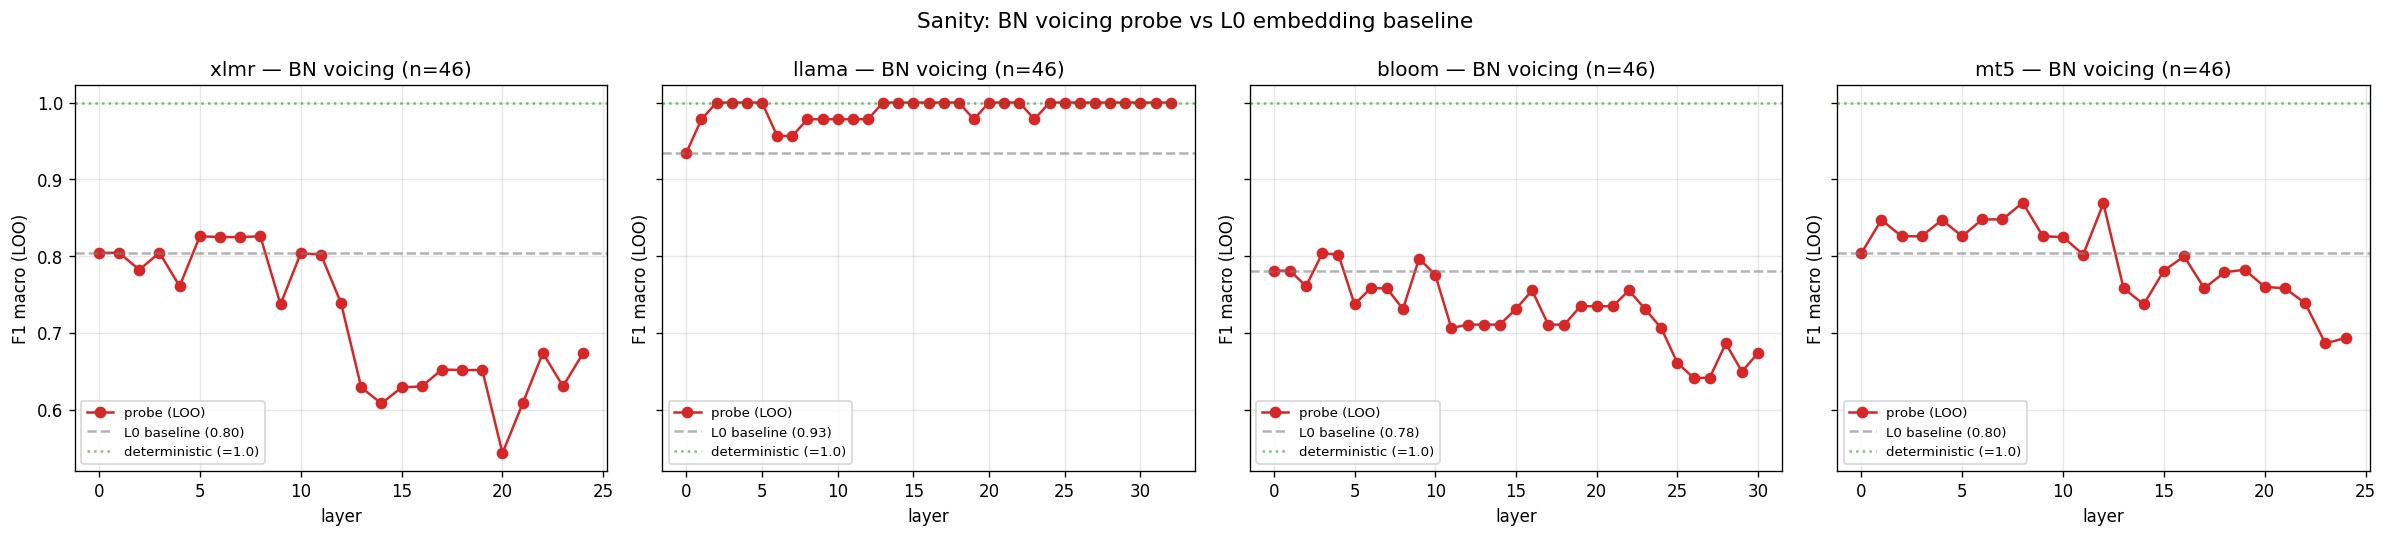
\includegraphics[width=0.96\columnwidth]{plots_bn_voicing_sanity.png}
\caption{Bangla voicing sanity check: a leave-one-out probe on layer-0 token embeddings recovers the voicing label at F1 0.78--0.94 across all four models, demonstrating that the label is inferable from first-character identity alone rather than from phonological voicing.}
\label{fig:voicing}
\end{figure}

\subsection{Length-matched recovery}
When real and pseudo words are matched 1:1 on character length, all four models exceed both their layer-0 and the five-feature surface baseline by at least $+0.20$ F1 on Bangla (Table~\ref{tab:realword}). This is the only task that passes the surface controls, and it is the basis for all subsequent transfer, RSA and ablation numbers. Figure~\ref{fig:emergence} shows the per-layer emergence trajectories across all four models and tasks; only the length-matched realword curves are interpretable.

\begin{table}[t]
\caption{Length-matched realword probing per language: layer-0 vs peak F1, with gain over layer~0. All four models gain $\geq +0.20$ on Bangla.}
\label{tab:realword}
\centering
\small
\setlength{\tabcolsep}{4pt}
\begin{tabular}{lcccccc}
\toprule
& \multicolumn{3}{c}{\textbf{English}} & \multicolumn{3}{c}{\textbf{Bangla}} \\
\cmidrule(lr){2-4}\cmidrule(lr){5-7}
\textbf{Model} & L0 & peak & gain & L0 & peak & gain \\
\midrule
XLM-R & 0.81 & 0.88 & $+0.06$ & 0.66 & 0.92 & $+0.25$ \\
Llama & 0.75 & 0.96 & $+0.21$ & 0.64 & 0.90 & $+0.26$ \\
BLOOM & 0.81 & 0.94 & $+0.13$ & 0.64 & 0.94 & $+0.30$ \\
mT5   & 0.65 & 0.90 & $+0.23$ & 0.72 & 0.92 & $+0.20$ \\
\bottomrule
\end{tabular}
\end{table}

\begin{figure*}[t]
\centering
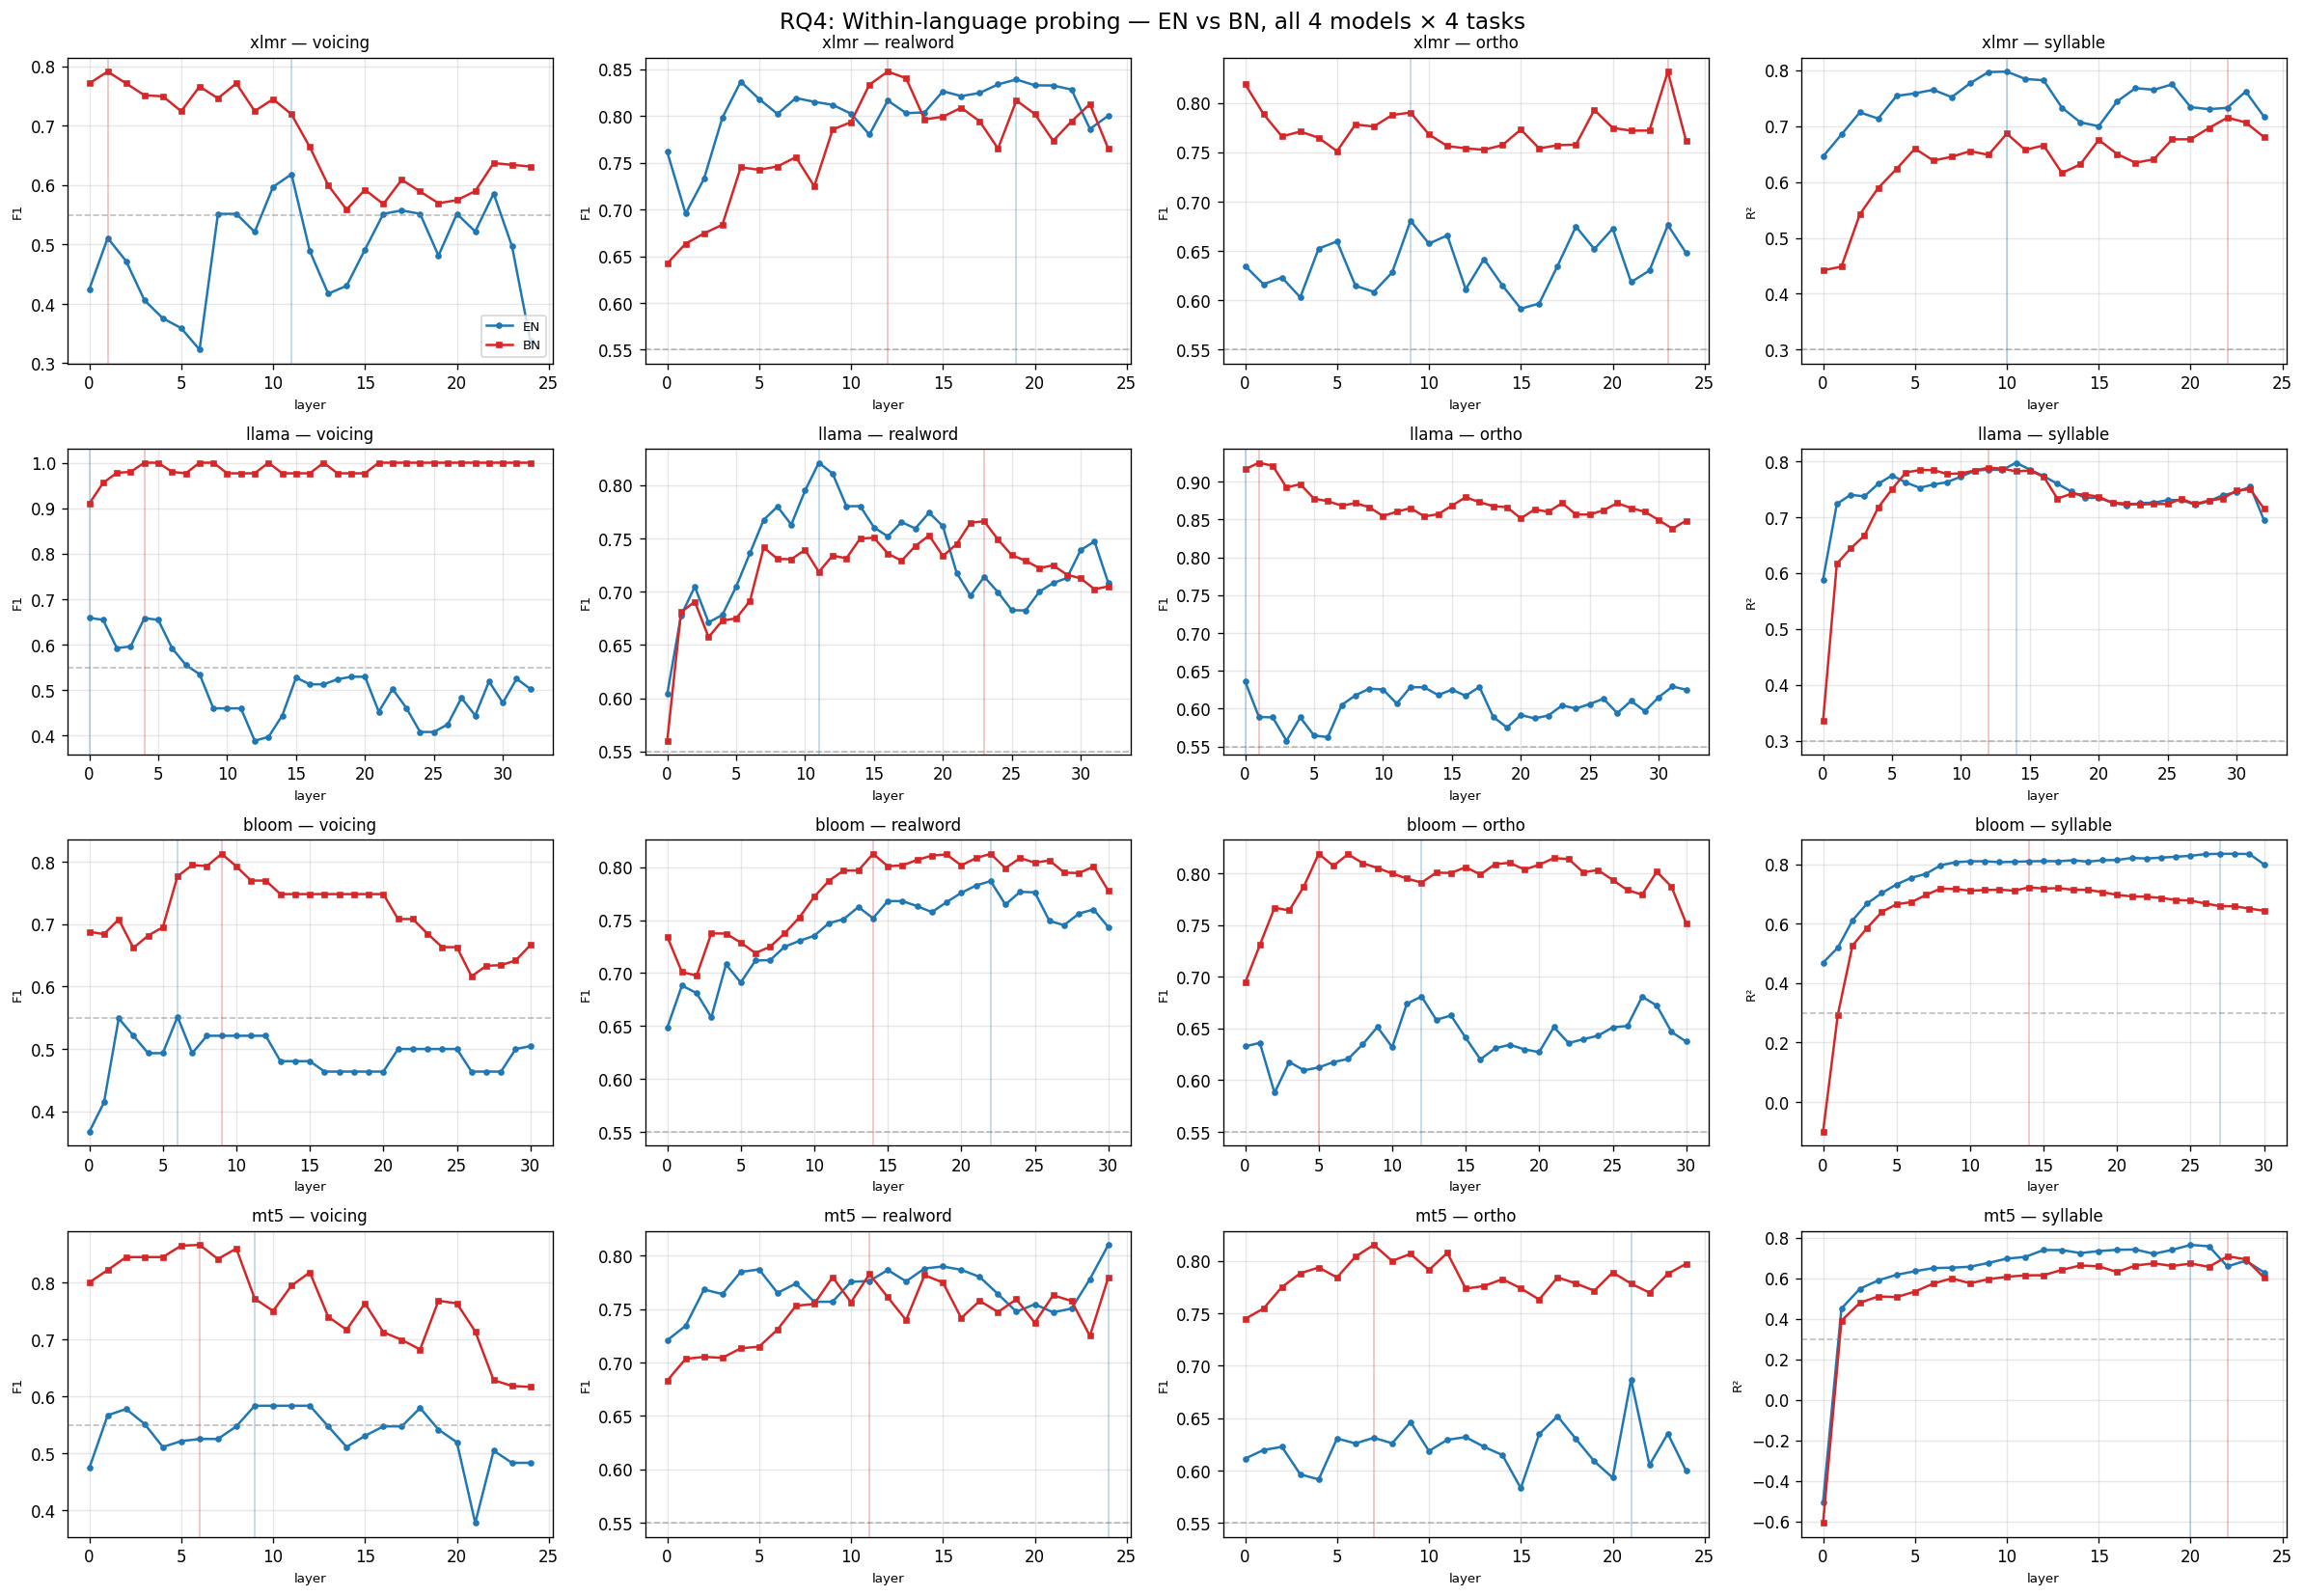
\includegraphics[width=0.92\textwidth]{plots_layer_emergence_all_models.png}
\caption{Per-layer emergence trajectories for the four models across the four tasks (layer axis normalised to relative encoder depth). The voicing, orthographic and syllable rows reflect surface confounds; only the length-matched realword row is an honest measurement.}
\label{fig:emergence}
\end{figure*}

\begin{figure}[t]
\centering
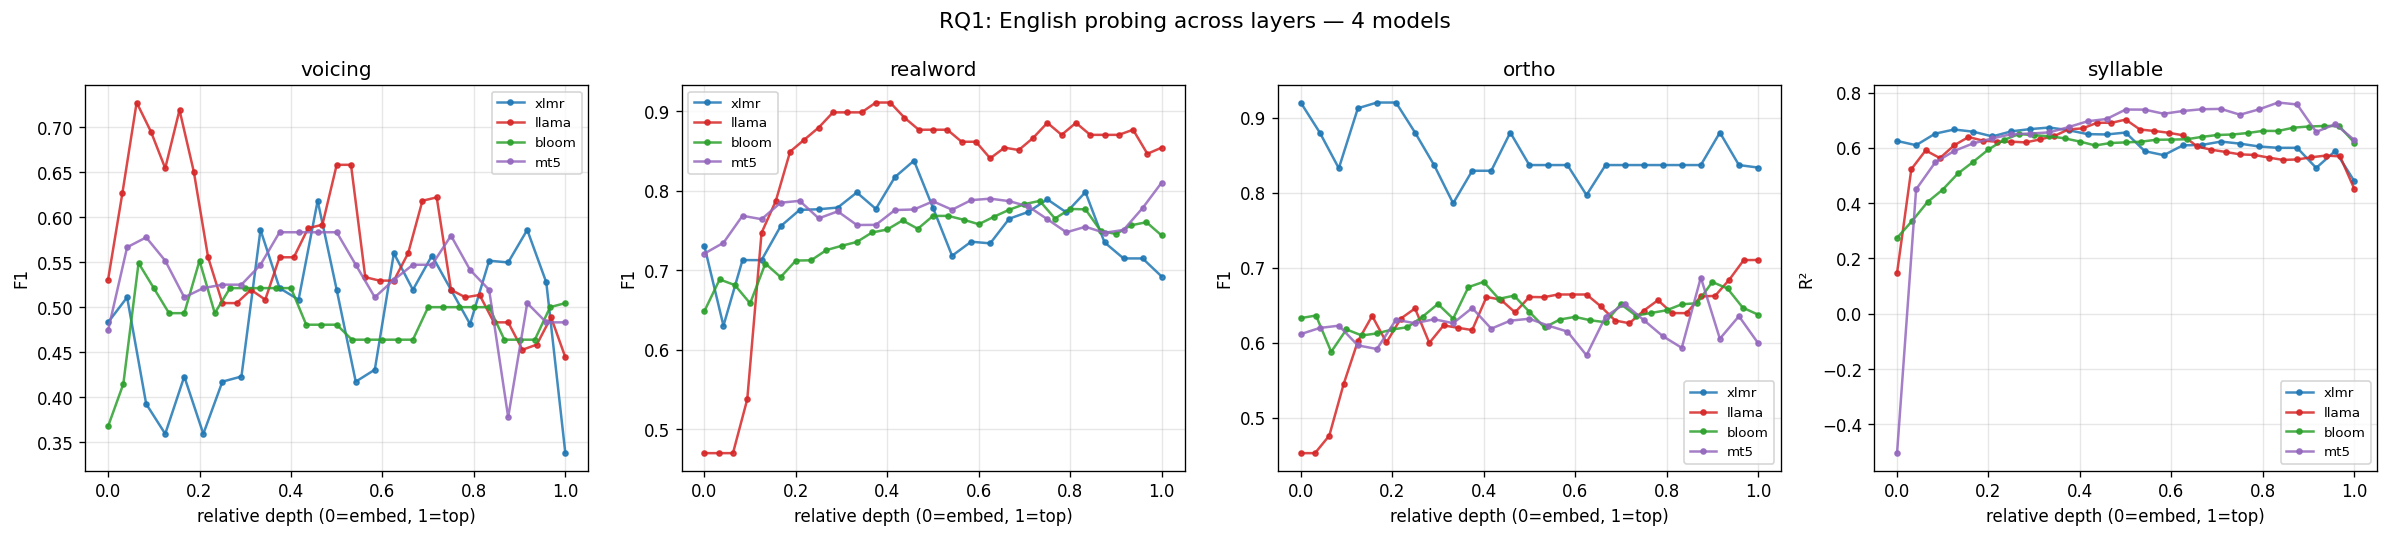
\includegraphics[width=0.96\columnwidth]{plots_four_models_english.png}
\caption{In-language English per-layer probing across the four models and four tasks. High in-language scores do not imply genuine phonological encoding once the surface-feature controls of Section~V-A are applied.}
\label{fig:english}
\end{figure}

\subsection{RQ2: cross-lingual transfer splits the models in two}
The English-trained length-matched realword probe, evaluated zero-shot on Bangla, cleanly separates the four models (Table~\ref{tab:results}, Fig.~\ref{fig:transfer}). BLOOM (0.92 F1, $+0.30$ over surface) and XLM-R (0.86 F1, $+0.24$) achieve genuine transfer, while Llama (0.63, $+0.01$) and mT5 (0.60, $-0.02$) collapse to surface level. Two implications follow. First, pretraining objective and language coverage \emph{jointly} determine transfer: BLOOM beats Llama at similar scale because it has explicit Bangla coverage, and the 0.56B XLM-R beats the 8B Llama at $\sim$13$\times$ fewer parameters. Architecture family alone is not predictive (XLM-R and BLOOM differ yet both transfer), and coverage alone is insufficient (mT5 is multilingual yet collapses; its span-corruption objective does not surface cross-lingual lexical similarity at the probe-readable level). Second, in-language English performance is not predictive of transfer: Llama has the highest English realword F1 (0.96) and the lowest Bangla transfer (0.63). The negative mT5 entry ($-0.02$) is not anti-learning; it means the representation scores marginally below the surface baseline, i.e.\ zero transfer within the $n=50$ estimation noise.

\begin{table*}[t]
\caption{Headline surface-controlled results. In-language and zero-shot cross-lingual real-versus-pseudo word F1 on the length-matched subset ($n{=}50$ per language), gain over the surface baseline, causal-ablation specificity, and the resulting role.}
\label{tab:results}
\centering
\small
\setlength{\tabcolsep}{4pt}
\begin{tabular}{lcccccl}
\toprule
\textbf{Model} & \textbf{In-lang BN F1} & \textbf{Transfer BN F1} & \textbf{Gain vs surface} & \textbf{Ablation spec.} & \textbf{Verdict} & \textbf{Recommended role} \\
\midrule
XLM-R large  & 0.92 & 0.86 & $+0.24$ & $+0.004$ (distrib.) & real transfer & efficiency (small GPU) \\
BLOOM 7B1    & 0.94 & \textbf{0.92} & \textbf{$+0.30$} & $-0.02$ (distrib.) & real transfer & best practical substrate \\
Llama 3.1 8B & 0.90 & 0.63 & $+0.01$ & n/a (BN chance) & collapsed & not recommended (Bangla) \\
mT5 XL       & 0.92 & 0.60 & $-0.02$ & \textbf{$+0.11$ (local.)} & collapsed & interpretability substrate \\
\bottomrule
\end{tabular}
\end{table*}

\begin{figure}[t]
\centering
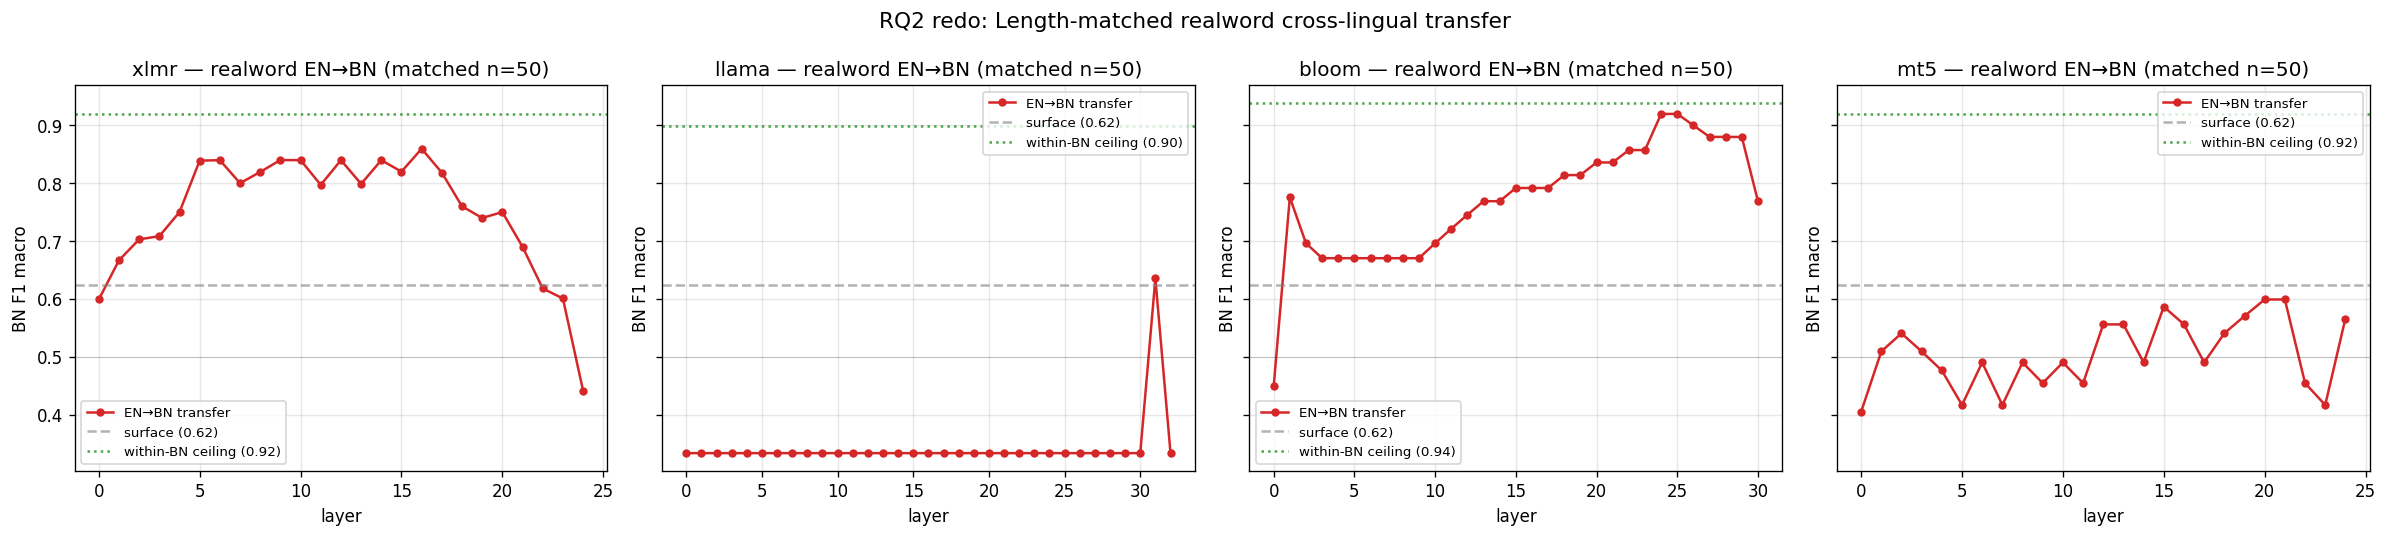
\includegraphics[width=0.96\columnwidth]{plots_transfer_realword_matched.png}
\caption{Surface-controlled length-matched real-vs-pseudo word cross-lingual transfer. XLM-R and BLOOM achieve genuine transfer ($+0.24$ and $+0.30$ over surface); Llama and mT5 collapse to surface level.}
\label{fig:transfer}
\end{figure}

\subsection{RSA corroborates the transfer split}
RSA agrees with the probing result. Cross-lingual RDM Spearman $\rho$ and English$\to$Bangla mate-retrieval Top-1 peak at mid layers for the transferring models; XLM-R reaches its highest cross-lingual RDM correlation in its middle encoder layers, coincident with the layer at which the length-matched realword probe transfers (L16). Llama reaches a high Top-1 in the \emph{unmatched} RSA setting, but this is driven by the same surface confound that inflates its unmatched probing numbers, and disappears under matching. Representational geometry is therefore preserved cross-lingually in XLM-R and BLOOM but not in mT5 (Table~\ref{tab:rsa}).

\begin{table}[t]
\caption{RSA summary: peak cross-lingual RDM Spearman $\rho$ and English$\to$Bangla mate-retrieval Top-1, with whether the signal survives length matching.}
\label{tab:rsa}
\centering
\small
\setlength{\tabcolsep}{5pt}
\begin{tabular}{lccc}
\toprule
\textbf{Model} & \textbf{Peak RDM $\rho$} & \textbf{Peak Top-1} & \textbf{Survives matching} \\
\midrule
XLM-R & mid-encoder & high & yes \\
BLOOM & mid layers  & 0.65 & yes \\
Llama & --          & 0.85$^\ast$ & no (surface) \\
mT5   & 0.244 (L15) & low  & no \\
\bottomrule
\end{tabular}
\\[2pt]
{\footnotesize $^\ast$Unmatched setting; driven by surface confound, vanishes under matching.}
\end{table}

\subsection{RQ3: only mT5 localises the signal}
Causal ablation distinguishes how the signal is stored (Table~\ref{tab:results}, Fig.~\ref{fig:ablation}). For mT5, zeroing the top-ranked encoder units selectively impairs Bangla transfer (specificity $+0.11$), whereas XLM-R and BLOOM are distributed (specificity near zero or marginally negative, indicating redundancy) and Llama has no transfer to disrupt. Repeating the ablation across five mT5 encoder depths (Table~\ref{tab:depth}) the effect persists at every depth and peaks at the mid-encoder (layer~12, specificity $+0.13$). The top-ranked sets overlap only partially across depths: two units (782 and 1880) recur in the top-10 at most depths and form a persistent backbone (Fig.~\ref{fig:backbone}), while 31 of 38 unique top-10 units are layer-specific. The mechanism is hybrid -- a small persistent backbone plus layer-local specialised circuits.

\begin{figure}[t]
\centering
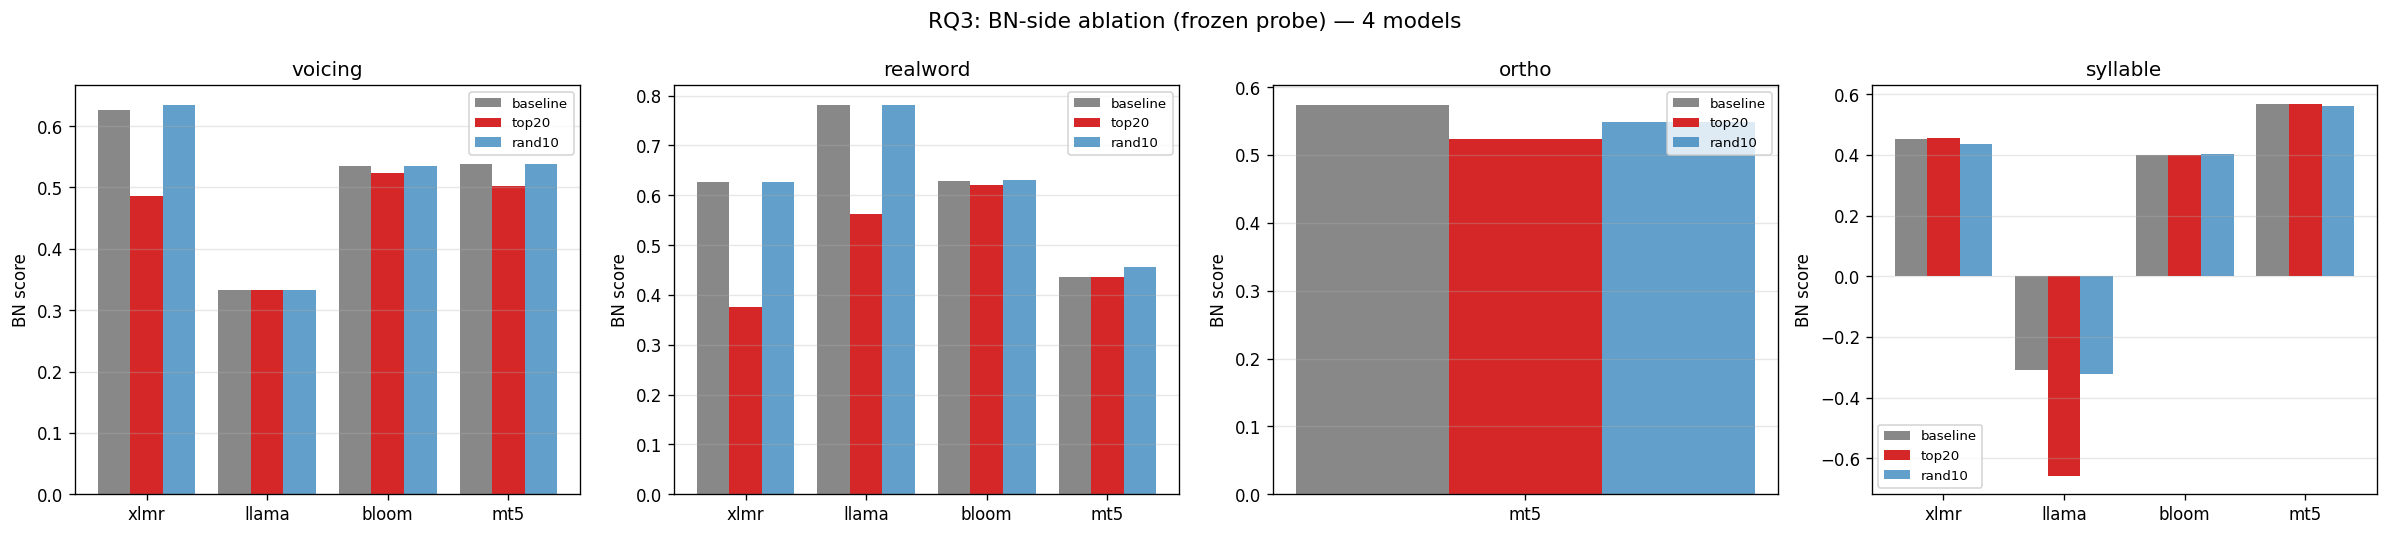
\includegraphics[width=0.96\columnwidth]{plots_four_models_ablation.png}
\caption{Four-model causal ablation on length-matched realword: top-$K$ versus random-$K$ unit ablation on the Bangla cross-lingual probe. Only mT5 shows clean specificity; XLM-R, BLOOM and Llama do not.}
\label{fig:ablation}
\end{figure}

\begin{table}[t]
\caption{mT5 encoder ablation across depth: top-10 vs random-mean specificity per \texttt{measure\_L} (three seeds). Localisation persists across depth; mid-encoder (L12) is strongest.}
\label{tab:depth}
\centering
\small
\setlength{\tabcolsep}{5pt}
\begin{tabular}{lcccc}
\toprule
\textbf{Depth} & \textbf{BN base} & \textbf{Top-10 drop} & \textbf{Rand mean} & \textbf{Specificity} \\
\midrule
L4  & 0.48 & $+0.06$ & $0.00$ & $+0.06$ \\
L8  & 0.49 & $+0.07$ & $0.00$ & $+0.07$ \\
\textbf{L12} & 0.56 & \textbf{$+0.14$} & $0.01$ & \textbf{$+0.13$} \\
L16 & 0.56 & $+0.03$ & $-0.01$ & $+0.04$ \\
L20 & 0.60 & $+0.11$ & $0.00$ & $+0.11$ \\
\bottomrule
\end{tabular}
\end{table}

\begin{figure}[t]
\centering
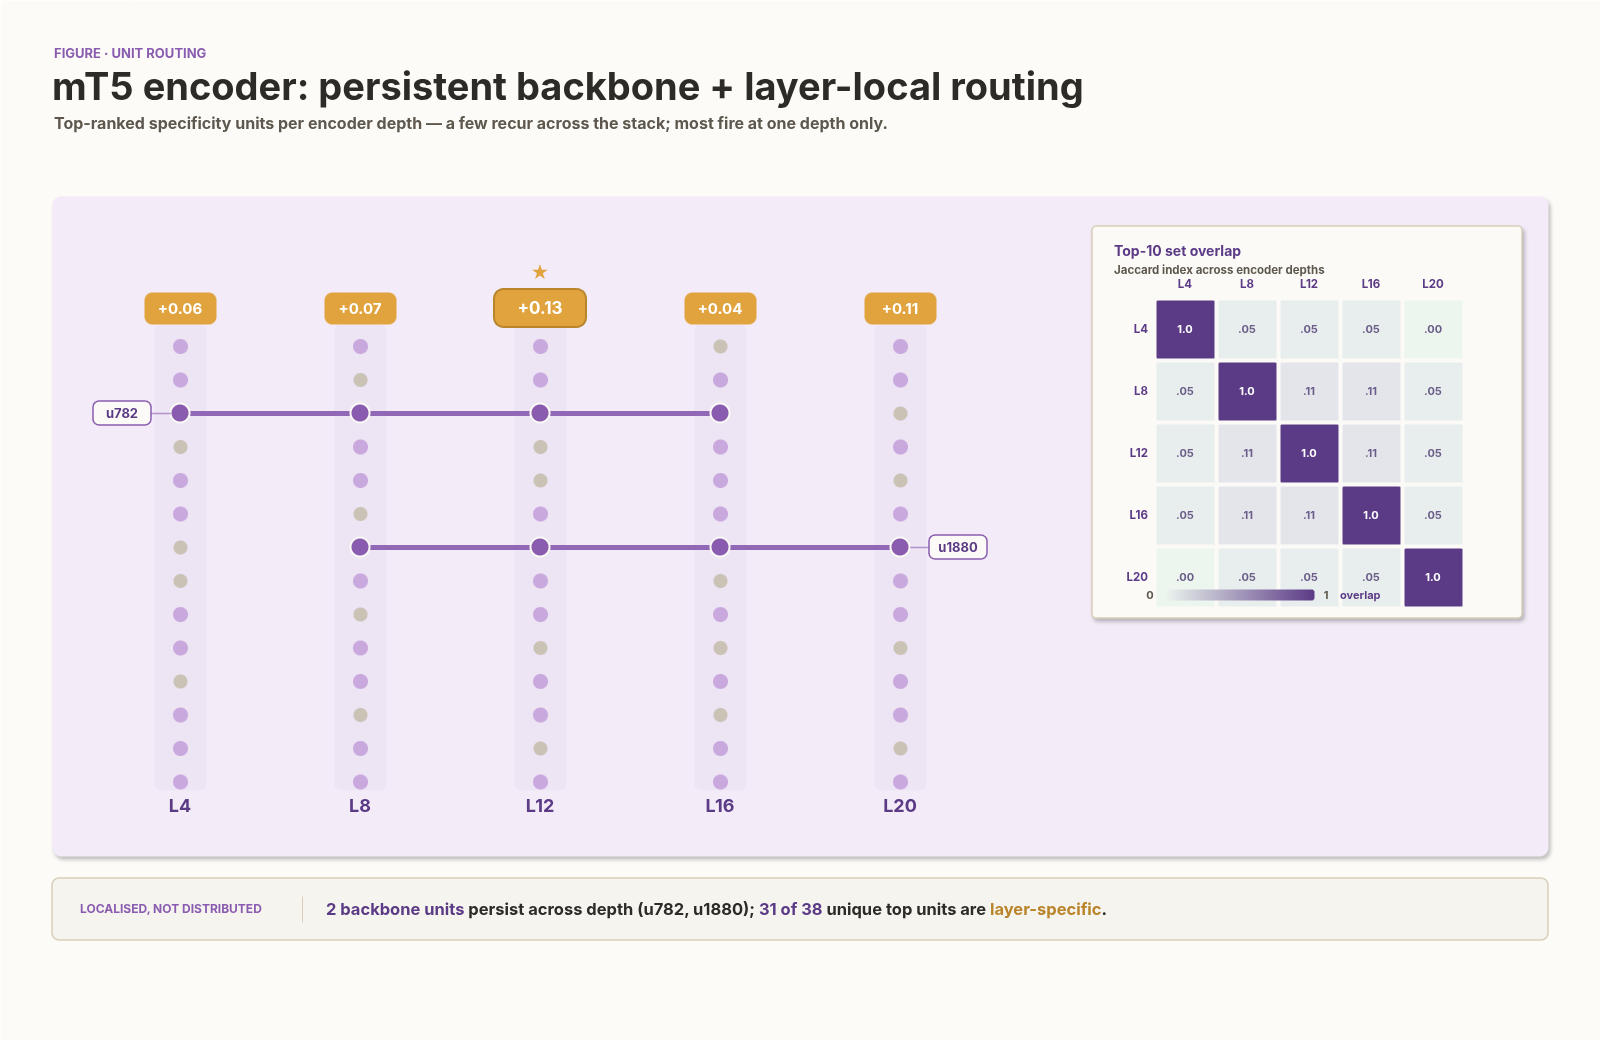
\includegraphics[width=0.96\columnwidth]{fig_mt5_backbone.png}
\caption{mT5 encoder localisation across depth. Two backbone units (u782, u1880) recur in the top-ranked set across most probed depths, while the remaining top units are layer-specific; per-depth ablation specificity peaks at L12. Inset: Jaccard overlap of the top-10 unit sets across depths.}
\label{fig:backbone}
\end{figure}

\subsection{RQ4: model selection}
No single model dominates every criterion. BLOOM is the best practical substrate for a Bangla screening prototype (highest transfer, 0.92 F1, $+0.30$); XLM-R is the most parameter-efficient (0.86 F1 at $\sim$13$\times$ fewer parameters); mT5 is the most interpretable (recoverable, localised mechanism); and Llama, despite being the largest, is not recommended for Bangla because its cross-lingual transfer collapses.

\section{Economic and Deployment Feasibility}
A practical advantage of frozen probing is cost. The full pipeline (four models $\times$ 440 stimuli $\times$ per-layer extraction, probing, RSA and ablation) runs in under 30 GPU-hours on a single consumer GPU, with no paid cloud-API expenditure; the marginal compute cost is on the order of BDT~120 in electricity, versus an estimated USD~110 for the representation-extraction stage alone via a hosted inference endpoint. Compared against training a comparable Bangla-only model from scratch ($\sim$50{,}000 GPU-hours and a $\geq 10^{10}$-token labelled Bangla corpus that does not exist), the frozen-prototype path is roughly $10^{3}$ cheaper on direct compute and qualitatively infinite on data. For a clinical pilot, the recommended BLOOM substrate serves at roughly 50 stimulus inferences per second under 4-bit quantisation; at 50 items per child and 1000 children per year, electricity is on the order of BDT~1500 per year, negligible relative to clinician time. This is the economic argument for defaulting to surface-controlled frozen probing of shared multilingual substrates in low-resource clinical-NLP settings before investing in any fine-tuning. Table~\ref{tab:cost} itemises the compute cost of the full pipeline.

\begin{table}[t]
\caption{Compute cost of the full DysLex-Probe pipeline on a single consumer GPU (electricity at BDT 11.5/kWh, 350~W average draw).}
\label{tab:cost}
\centering
\small
\setlength{\tabcolsep}{5pt}
\begin{tabular}{lcc}
\toprule
\textbf{Pipeline stage} & \textbf{GPU-hours} & \textbf{Elec.\ (BDT)} \\
\midrule
Representation extraction & 16 & 64 \\
Per-layer probing & 4 & 16 \\
Surface sanity checks & 1 & 4 \\
RSA & 2 & 8 \\
Causal ablation & 3 & 12 \\
mT5 depth-scan ($5\times3$ seeds) & 4 & 16 \\
\midrule
\textbf{Total} & \textbf{30} & \textbf{$\sim$120} \\
\bottomrule
\end{tabular}
\end{table}

\section{Discussion}
The results yield one practical and one methodological lesson. Practically, for low-resource cross-lingual lexical work, multilingual coverage and pretraining objective matter more than parameter scale: a small multilingual encoder beats a much larger English-heavy decoder, and the best transfer comes from a multilingual decoder with explicit coverage. This inverts the common heuristic of selecting the largest available model, and it gives downstream builders a concrete starting point.

Methodologically, the surface-feature controls overturn three of four standard tasks. The voicing result is the sharpest: a label that looks phonological is fully recoverable from the first character, so any apparent voicing success is letter recognition. This implies that prior cross-lingual phonological probing results obtained without surface matching may overstate phonological encoding. The fact that real-versus-pseudoword discrimination survives, and survives across all four models, indicates that genuine cross-lingual lexical structure does exist once confounds are removed.

Finally, the mT5 localisation result is of independent interpretability interest: an encoder-decoder trained with span corruption concentrates cross-lingual lexical information into a handful of units with a stable backbone, while encoder-only and decoder-only models distribute it. This suggests the pretraining objective shapes not only \emph{whether} cross-lingual structure forms but \emph{how} it is organised.

A further implication concerns the interpretation of prior cross-lingual phonological probing. Because three of our four tasks are solved by surface cues, results in the literature reporting strong cross-lingual phonological encoding without stimulus-level surface matching may, in part, reflect character statistics or token identity rather than transferable phonology. Our positive result -- that real-versus-pseudoword discrimination survives across all four models after matching -- is therefore the more conservative and more trustworthy claim: it is precisely the task that cannot be reduced to length or first-character cues, and it is the task most directly tied to the behavioural marker of dyslexia. The practical and methodological lessons reinforce each other: the same surface controls that invalidate three tasks are what make the surviving cross-lingual transfer credible enough to base a model-selection recommendation on.

Although our target is Bangla, the design generalises to other low-resource languages. The method requires only (i) a small, surface-matched, native-verified stimulus set in the target language, paired with an English source, and (ii) a frozen multilingual model with explicit coverage of that target. The first-character and character-statistic controls are language-agnostic and would expose analogous confounds in, for example, Devanagari or Tamil scripts. Because the substrate is shared and frozen, the embodied cost of building screening prototypes is amortised across many languages, which is the central efficiency argument for this approach over per-language pretraining or fine-tuning.

\section{Limitations and Ethical Considerations}
This is a representational probe, not a clinical instrument: a model scoring 0.92 F1 on a research task cannot diagnose dyslexia, and deploying it as if it could would harm children through false positives and false negatives. Clinician-supervised validation with real readers is required before any deployment. The length-matched subset is small ($n=50$ per language), so per-layer scores are point estimates rather than confidence intervals. mT5 is the only encoder-decoder tested, so its localisation could reflect the span-corruption objective, the encoder-decoder split, or both; disentangling these requires more encoder-decoder models. The dataset uses standard Bangla forms and does not capture dialectal variation. The dataset is original and contains no human-participant data; all model weights are used in a frozen, read-only manner under their published licences.

\section{Future Work}
Three directions follow. First, enlarge and diversify the Bangla data, including dialects and broader conjunct coverage, and report confidence intervals. Second, advance from probing to a clinician-supervised screening pilot built on the recommended BLOOM substrate, evaluated with real children and experts. Third, extend the localisation analysis to additional encoder-decoder models to resolve the architecture-versus-objective confound, and design future labels so that they cannot be shortcut by surface features.

\section{Conclusion}
We probed four multilingual LLMs spanning the dominant pretraining recipes for cross-lingual lexical structure relevant to low-resource Bangla dyslexia screening, under strict surface controls. Three of four standard probing tasks measure surface shortcuts; once corrected, BLOOM and XLM-R carry genuine English-to-Bangla transfer while a larger English-heavy decoder does not, and mT5 uniquely localises the signal. The work delivers both a principled model-selection recommendation for low-resource Bangla screening and a reusable surface-control methodology that should be the minimum standard for clinical probing of multilingual models.

\begin{thebibliography}{00}
\bibitem{snowling2020dyslexia} M.~J. Snowling, C.~Hulme, and K.~Nation, ``Defining and understanding dyslexia: past, present and future,'' \emph{Oxford Review of Education}, vol.~46, no.~4, pp.~501--513, 2020.
\bibitem{peterson2012developmental} R.~L. Peterson and B.~F. Pennington, ``Developmental dyslexia,'' \emph{The Lancet}, vol.~379, no.~9830, pp.~1997--2007, 2012.
\bibitem{ziegler2005reading} J.~C. Ziegler and U.~Goswami, ``Reading acquisition, developmental dyslexia, and skilled reading across languages: a psycholinguistic grain size theory,'' \emph{Psychological Bulletin}, vol.~131, no.~1, pp.~3--29, 2005.
\bibitem{wagner2020prevalence} R.~K. Wagner \emph{et al.}, ``The prevalence of dyslexia: a new approach to its estimation,'' \emph{Journal of Learning Disabilities}, vol.~53, no.~5, pp.~354--365, 2020.
\bibitem{goswami2011temporal} U.~Goswami, ``A temporal sampling framework for developmental dyslexia,'' \emph{Trends in Cognitive Sciences}, vol.~15, no.~1, pp.~3--10, 2011.
\bibitem{wagner2013ctopp} R.~K. Wagner, J.~K. Torgesen, C.~A. Rashotte, and N.~A. Pearson, \emph{Comprehensive Test of Phonological Processing (CTOPP-2)}. Austin, TX: PRO-ED, 2013.
\bibitem{nag2014dyslexia} S.~Nag and M.~J. Snowling, ``Children's reading development: learning about sounds, symbols and cross-modal mappings,'' \emph{WIREs Cognitive Science}, vol.~5, no.~6, pp.~681--690, 2014.
\bibitem{nag2017indian} S.~Nag, ``Learning to read Kannada and other languages of South Asia,'' in \emph{Reading Development and Difficulties}, Springer, 2017.
\bibitem{badsha2024mall} M.~S. Badsha, ``Mobile assisted language learning (MALL) tools for Bengali dyslexic primary school students,'' \emph{Int. J. for Multidisciplinary Research (IJFMR)}, vol.~6, no.~3, 2024.
\bibitem{conneau2020xlmr} A.~Conneau \emph{et al.}, ``Unsupervised cross-lingual representation learning at scale,'' in \emph{Proc. 58th Annu. Meeting Assoc. Comput. Linguistics (ACL)}, 2020, pp.~8440--8451.
\bibitem{scao2022bloom} T.~Le~Scao \emph{et al.}, ``BLOOM: a 176B-parameter open-access multilingual language model,'' \emph{arXiv:2211.05100}, 2022.
\bibitem{xue2021mt5} L.~Xue \emph{et al.}, ``mT5: a massively multilingual pre-trained text-to-text transformer,'' in \emph{Proc. NAACL-HLT}, 2021, pp.~483--498.
\bibitem{dubey2024llama3} A.~Dubey \emph{et al.}, ``The Llama 3 herd of models,'' \emph{arXiv:2407.21783}, 2024.
\bibitem{pires2019mbert} T.~Pires, E.~Schlinger, and D.~Garrette, ``How multilingual is multilingual BERT?,'' in \emph{Proc. ACL}, 2019, pp.~4996--5001.
\bibitem{wu2020emerging} S.~Wu and M.~Dredze, ``Are all languages created equal in multilingual BERT?,'' in \emph{Proc. 5th Workshop Representation Learning for NLP (RepL4NLP)}, 2020, pp.~120--130.
\bibitem{conneau2018probing} A.~Conneau, G.~Kruszewski, G.~Lample, L.~Barrault, and M.~Baroni, ``What you can cram into a single vector: probing sentence embeddings for linguistic properties,'' in \emph{Proc. ACL}, 2018, pp.~2126--2136.
\bibitem{hewitt2019structural} J.~Hewitt and C.~D. Manning, ``A structural probe for finding syntax in word representations,'' in \emph{Proc. NAACL-HLT}, 2019, pp.~4129--4138.
\bibitem{belinkov2022probing} Y.~Belinkov, ``Probing classifiers: promises, shortcomings, and advances,'' \emph{Computational Linguistics}, vol.~48, no.~1, pp.~207--219, 2022.
\bibitem{pimentel2020information} T.~Pimentel, J.~Valvoda, R.~H. Maudslay, R.~Zmigrod, A.~Williams, and R.~Cotterell, ``Information-theoretic probing for linguistic structure,'' in \emph{Proc. ACL}, 2020, pp.~4609--4622.
\bibitem{dettmers2022bnb} T.~Dettmers, M.~Lewis, Y.~Belkada, and L.~Zettlemoyer, ``LLM.int8(): 8-bit matrix multiplication for transformers at scale,'' in \emph{Adv. Neural Inf. Process. Syst. (NeurIPS)}, 2022.
\end{thebibliography}

\end{document}
